% !TEX TS-program = XeLaTeX
% use the following command: 
% all document files must be coded in UTF-8
\documentclass{textolivre}
% for anonymous submission
%\documentclass[anonymous]{textolivre}
% to create HTML use 
%\documentclass{textolivre-html}
% See more information on the repository: https://github.com/leolca/textolivre

% Metadata
\begin{filecontents*}[overwrite]{article.xmpdata}
    \Title{El engagement en la educación virtual: experiencias durante la pandemia COVID-19}
    \Author{Odiel Estrada Molina \sep Dieter Reynaldo Fuentes Cancell \sep Alién García Hernández}
    \Language{es}
    \Keywords{Cuasi-experimento \sep Cursos virtuales \sep Covid-19 \sep Engagement \sep Tecnología educativa}
    \Journaltitle{Texto Livre}
    \Journalnumber{1983-3652}
    \Volume{14}
    \Issue{2}
    \Firstpage{1}
    \Lastpage{18}
    \Doi{10.35699/1983-3652.2021.33936}

    \setRGBcolorprofile{sRGB_IEC61966-2-1_black_scaled.icc}
            {sRGB_IEC61966-2-1_black_scaled}
            {sRGB IEC61966 v2.1 with black scaling}
            {http://www.color.org}
\end{filecontents*}

% used to create dummy text for the template file
\definecolor{dark-gray}{gray}{0.35} % color used to display dummy texts
\usepackage{lipsum}
\SetLipsumParListSurrounders{\colorlet{oldcolor}{.}\color{dark-gray}}{\color{oldcolor}}

% used here only to provide the XeLaTeX and BibTeX logos
\usepackage{hologo}

% used in this example to provide source code environment
%\crefname{lstlisting}{lista}{listas}
%\Crefname{lstlisting}{Lista}{Listas}
%\usepackage{listings}
%\renewcommand\lstlistingname{Lista}
%\lstset{language=bash,
        breaklines=true,
        basicstyle=\linespread{1}\small\ttfamily,
        numbers=none,xleftmargin=0.5cm,
        frame=none,
        framexleftmargin=0.5em,
        framexrightmargin=0.5em,
        showstringspaces=false,
        upquote=true,
        commentstyle=\color{gray},
        literate=%
           {á}{{\'a}}1 {é}{{\'e}}1 {í}{{\'i}}1 {ó}{{\'o}}1 {ú}{{\'u}}1 
           {à}{{\`a}}1 {è}{{\`e}}1 {ì}{{\`i}}1 {ò}{{\`o}}1 {ù}{{\`u}}1
           {ã}{{\~a}}1 {ẽ}{{\~e}}1 {ĩ}{{\~i}}1 {õ}{{\~o}}1 {ũ}{{\~u}}1
           {â}{{\^a}}1 {ê}{{\^e}}1 {î}{{\^i}}1 {ô}{{\^o}}1 {û}{{\^u}}1
           {ä}{{\"a}}1 {ë}{{\"e}}1 {ï}{{\"i}}1 {ö}{{\"o}}1 {ü}{{\"u}}1
           {Á}{{\'A}}1 {É}{{\'E}}1 {Í}{{\'I}}1 {Ó}{{\'O}}1 {Ú}{{\'U}}1
           {À}{{\`A}}1 {È}{{\`E}}1 {Ì}{{\`I}}1 {Ò}{{\`O}}1 {Ù}{{\`U}}1
           {Ã}{{\~A}}1 {Ẽ}{{\~E}}1 {Ũ}{{\~u}}1 {Õ}{{\~O}}1 {Ũ}{{\~U}}1
           {Â}{{\^A}}1 {Ê}{{\^E}}1 {Î}{{\^I}}1 {Ô}{{\^O}}1 {Û}{{\^U}}1
           {Ä}{{\"A}}1 {Ë}{{\"E}}1 {Ï}{{\"I}}1 {Ö}{{\"O}}1 {Ü}{{\"U}}1
           {ç}{{\c{c}}}1 {Ç}{{\c{C}}}1
}


\journalname{Texto Livre}
\thevolume{14}
\thenumber{2}
\theyear{2021}
\receiveddate{\DTMdisplaydate{2020}{12}{11}{-1}} % YYYY MM DD
\accepteddate{\DTMdisplaydate{2021}{02}{28}{-1}}
\publisheddate{\DTMdisplaydate{2021}{06}{28}{-1}}
% Corresponding author
\corrauthor{Odiel Estrada Molina}
% DOI
\articledoi{10.35699/1983-3652.2021.33936}
% list of available sesscions in the journal: articles, dossier, reports, essays, reviews, interviews, editorial
\articlesessionname{dossier}
% Abbreviated author list for the running footer
\runningauthor{Estrada Molina et al}
\editorname{Anna Izabella Miranda Pereira}

\title{El \textit{engagement} en la educación virtual: experiencias durante la pandemia COVID-19}
\othertitle{Engajamento na educação virtual: experiências durante a pandemia de COVID-19}
\othertitle{Engagement in virtual education: experiences during the COVID-19 pandemic}
% if there is a third language title, add here:
%\othertitle{Artikelvorlage zur Einreichung beim Texto Livre Journal}

\author[1]{Odiel Estrada Molina \orcid{0000-0002-0918-418X} \thanks{Email: \url{oestrada@uci.cu}}}
\author[1]{Dieter Reynaldo Fuentes Cancell \orcid{0000-0002-2509-5400} \thanks{Email: \url{dieterr@uci.cu}}}
\author[1]{Alién García Hernández \orcid{0000-0002-9701-9351} \thanks{Email: \url{agarciahh@uci.cu}}}

\affil[1]{Facultad de Ciencias y Tecnologías Computacionales. Universidad de las Ciencias Informáticas, La Habana, Cuba.}

\addbibresource{article.bib}
% use biber instead of bibtex
% $ biber tl-article-template

% set language of the article
\setdefaultlanguage{spanish}
\setotherlanguage{portuguese}
\setotherlanguage{english}

% for spanish, use:
%\setdefaultlanguage{spanish}
\gappto\captionsspanish{\renewcommand{\tablename}{Tabla}} % use 'Tabla' instead of 'Cuadro'
\AfterEndPreamble{\crefname{table}{tabla}{tablas}\Crefname{table}{Tabla}{Tablas}}

% for languages that use special fonts, you must provide the typeface that will be used
% \setotherlanguage{arabic}
% \newfontfamily\arabicfont[Script=Arabic]{Amiri}
% \newfontfamily\arabicfontsf[Script=Arabic]{Amiri}
% \newfontfamily\arabicfonttt[Script=Arabic]{Amiri}
%
% in the article, to add arabic text use: \textlang{arabic}{ ... }

% to use emoticons in your manuscript
% https://stackoverflow.com/questions/190145/how-to-insert-emoticons-in-latex/57076064
% using font Symbola, which has full support
% the font may be downloaded at:
% https://dn-works.com/ufas/
% add to preamble:
% \newfontfamily\Symbola{Symbola}
% in the text use:
% {\Symbola }

% reference itens in a descriptive list using their labels instead of numbers
% insert the code below in the preambule:
\makeatletter
\let\orgdescriptionlabel\descriptionlabel
\renewcommand*{\descriptionlabel}[1]{%
  \let\orglabel\label
  \let\label\@gobble
  \phantomsection
  \edef\@currentlabel{#1\unskip}%
  \let\label\orglabel
  \orgdescriptionlabel{#1}%
}
\makeatother
%
% in your document, use as illustraded here:
%\begin{description}
%  \item[first\label{itm1}] this is only an example;
%  % ...  add more items
%\end{description}
 

% custom epigraph - BEGIN 
%%% https://tex.stackexchange.com/questions/193178/specific-epigraph-style
\usepackage{epigraph}
\renewcommand\textflush{flushright}
\makeatletter
\newlength\epitextskip
\pretocmd{\@epitext}{\em}{}{}
\apptocmd{\@epitext}{\em}{}{}
\patchcmd{\epigraph}{\@epitext{#1}\\}{\@epitext{#1}\\[\epitextskip]}{}{}
\makeatother
\setlength\epigraphrule{0pt}
\setlength\epitextskip{0.5ex}
\setlength\epigraphwidth{.7\textwidth}
% custom epigraph - END


% if you use multirows in a table, include the multirow package
\usepackage{multirow}

% add line numbers for submission
%\usepackage{lineno}
%\linenumbers

\begin{document}
\maketitle

\begin{polyabstract}
\begin{abstract}
Los cursos virtuales son alternativas educativas que contribuyen a la formación permanente de los profesionales. Lograr un adecuado \emph{engagement} permite elevar la motivación, compromiso, responsabilidad y emociones positivas hacia el logro de los objetivos y metas de aprendizaje. Debido a las actuales condiciones de confinamiento provocado por la pandemia Covid-19 es imprescindible lograr un \emph{engagement} en los cursos virtuales. Este estudio tiene como objetivo determinar si el rediseño del curso virtual Introducción a la Evaluación de la Usabilidad de Sistemas Informáticos, ofertado en la Universidad de las Ciencias Informáticas de Cuba propicia mayores niveles de \emph{engagement} en las actuales condiciones de confinamiento. Se diseñó un cuasi-experimento con un grupo de control y uno experimental. Las pruebas estadísticas confirman mayores niveles de \emph{engagement} en los sujetos del grupo experimental. Se concluye que, las características a potenciar en los cursos virtuales ofertados en el actual tiempo de pandemia para elevar el \emph{engagement} son: (1) factor \emph{engagement} aplicado: diseño de recursos educativos digitales y materiales relevantes para la vida profesional y, aplicación de lo aprendido; (2) Factor \emph{engagement} orientado a objetivos: integración entre el clima psicológico organizacional y la motivación profesional y, actividades colaborativas; y (3) Factor \emph{engagement} autodisciplinado y el \emph{engagement} interactivo: contenidos «desafiantes» de aprendizaje, actividades sincrónicas y asincrónica y sesiones interactivas a través de Telegram.


\keywords{Cuasi-experimento \sep Cursos virtuales \sep Covid-19 \sep \emph{Engagement} \sep Tecnología educativa}
\end{abstract}

\begin{portuguese}
\begin{abstract}
Os cursos a distância são alternativas educacionais que contribuem para a formação permanente dos profissionais. Alcançar um engajamento adequado permite aumentar a motivação, o comprometimento, a responsabilidade e as emoções positivas em relação ao cumprimento dos objetivos e metas de aprendizagem. Devido às atuais condições de confinamento causadas pela pandemia Covid-19, é essencial conseguir o envolvimento em cursos virtuais. O objetivo deste estudo é determinar se o redesenho do curso virtual "Introdução à avaliação da usabilidade de sistemas computacionais", oferecido pela Universidad de las Ciencias Informáticas, favorece níveis mais elevados de engajamento nas atuais condições de confinamento. Um quase-experimento foi projetado com um grupo de controle e um grupo experimental. Os testes estatísticos confirmam níveis mais elevados de engajamento nos sujeitos do grupo experimental. Conclui-se com base nas experiências educacionais obtidas que as características a serem promovidas nos cursos a distância oferecidos no momento atual da pandemia para aumentar o engajamento são: (1) fator de engajamento aplicado: desenho de recursos educacionais digitais e materiais relevantes para a vida profissional e aplicação do que foi aprendido; (2) Fator de engajamento orientado a metas: integração entre o clima psicológico organizacional e a motivação profissional e atividades colaborativas; e (3) Fator de engajamento autodisciplinado e engajamento interativo: conteúdo de aprendizagem "desafiador", atividades síncronas, e assíncronas e sessões interativas por meio do Telegram.

\keywords{Quase-experimento \sep Cursos virtuais \sep Covid-19 \sep Engajamento \sep Tecnologia educacional}
\end{abstract}
\end{portuguese}

\begin{english}
\begin{abstract}
Virtual courses are educational alternatives that contribute to the permanent training of professionals. Achieving adequate engagement allows raising motivation, commitment, responsibility, and positive emotions towards the achievement of learning objectives and goals. Due to the current confinement conditions caused by the Covid-19 pandemic, it is essential to achieve, as far as possible, an engagement in the virtual courses. The objective of this study is to determine if the redesign of the virtual course "Introduction to the evaluation of the usability of computer systems" offered at the Universidad de las Ciencias Informáticas favors higher levels of engagement in the current confinement conditions. A quasi-experiment was designed with a control group and an experimental group. Statistical tests confirm higher levels of engagement in the subjects of the experimental group. It is concluded based on the educational experiences obtained that the characteristics that should be promoted in the virtual courses offered in the current time of the pandemic are (1) applied engagement factor: design of digital educational resources and relevant materials for professional life and application of what has been learned; (2) Goal-oriented engagement factor: integration between the organizational psychological climate and professional motivation, and collaborative activities; and (3) Self-disciplined engagement factor and interactive engagement: challenging learning content, synchronous and asynchronous activities, and interactive sessions through Telegram.

\keywords{Quasi-experiment \sep Virtual courses \sep Covid-19 \sep Engagement \sep Educational Technology}
\end{abstract}
\end{english}

% if there is another abstract, insert it here using the same scheme
\end{polyabstract}


\section{Introducción}\label{intro}
La pandemia de la Covid-19 obliga que en los distintos países se apliquen diversas medidas sociales, económicas y políticas con el propósito, dentro de lo posible, de salvaguardar la vida humana. Estos cambios inciden en diversos sectores estratégicos, siendo uno de ellos la educación universitaria.

Las universidades en los últimos 20 años potencian la educación virtual como alternativa para la sistematización de competencias, la superación profesional en correspondencia a las actuales desafíos y demandas laborales, así como la masificación de la educación (gratis o no). En esta modalidad educativa los recursos educativos digitales, la tutoría y rol participativo, interactivo y colaborativo de los docentes y estudiantes a través de los entornos virtuales cobran una mayor relevancia en el proceso de enseñanza-aprendizaje.

En este escenario están presentes disímiles variables que atentan, en cierta medida, con un adecuado rendimiento de los estudiantes, entre ellas, el \emph{engagement}. Este concepto se relaciona con el compromiso, bienestar, motivación y la persistencia que tiene el alumnado en los estudios \cite{schaufeli2002}. %(SCHAUFELI; MARTÍNEZ; PINTO; SALANOVA; BAKKER, 2002). 
Estos factores toman especial relevancia en la educación virtual, en la cual diversos profesionales tienen una alternativa de superación constante en correspondencia a sus necesidades de aprendizaje.

Debido al comentario anterior referente a la pandemia, es notable un aumento de trabajadores que acceden a cursos virtuales en las universidades para aprender o certificar sus conocimientos y poder así, mejorar su status laboral y condiciones socioeconómicas. Sin embargo, sus condiciones económicas y de conectividad inciden en el \emph{engagement} hacia los cursos virtuales.

Diversos estudios se publicaron en el último año referentes a la educación en tiempos de la pandemia Covid-19. \textcite{cacerespinaloza2020} %CÁCERES-PIÑALOZA (2020)
argumenta la importancia de los espacios afectivos; \textcite{kemmekah2020, jordan2020, lin2020, hernandezramos2021} %KEM-MEKAH, (2020); JORDAN, DAVID; PHILLIPS; PELLINI(2020);  LIN; REIGELUTH (2020) y HERNÁNDEZ-RAMOS; MARTÍNEZ-ABAD; SÁNCHEZ-PRIETO (2021) 
transmiten sus experiencias a partir de la interactividad con los recursos educativos digitales; otras investigaciones establecen los desafíos educativos actuales ante la Covid-19 \cite{baptistalucio2020, miguel2020, floresnessi2020, velasquez2020, jimenez2021} %(BAPTISTA; ALMAZÁN; LOEZA, 2020; MIGUEL, 2020;  FLORES; MELÉNDEZ; BAPTISTA, 2020; VELÁSQUEZ, 2020; JIMÉNEZ; RUIZ, 2021)
mientras que diversos autores exponen las principales preocupaciones motivacionales de los matriculados en cursos virtuales \cite{diazguillen2018, ojeda2020, valdivieso2020, gonzalez2020}. %(DÍAZ; ANDRADE; URIBE, 2020; OJEDA; ORTEGA; BOOM, 2020; VALDIVIESO, BURBANO; BURBANO, 2020; GONZÁLEZ, 2020).
Coherente con estas últimas investigaciones, se aborda la relación entre el rendimiento académico, \emph{engagement} y el estrés causado por el confinamiento que viven la mayoría de las personas \cite{alvarezherrero-hernandez2020, hernandez2020, mahdy2020, valdivieso2020, santiagoiglesias2021}. %(ÁLVAREZ-HERRERO; HERNÁNDEZ-ORTEGA, 2020; HERNÁNDEZ, 2020; MAHDY, 2020;  VALDIVIESO; BURBANO; BURBANO, 2020; SANTIAGO; HERNÁNDEZ-GARCÍA; CHAPARRO-PELÁEZ; PRIETO, 2021).

El análisis bibliográfico realizado refleja que pocas investigaciones (inicios del 2020-actualidad febrero de 2021) abordan las experiencias educativas ante la Covid-19 desde las condiciones tecnológicas, económicas y educativas de países en subdesarrollo. Por tal motivo, en esta investigación de carácter exploratorio se tiene como objetivo primario determinar si el rediseño del curso virtual Introducción a la Evaluación de la Usabilidad de Sistemas Informáticos que oferta la Universidad de las Ciencias Informáticas de Cuba propicia mayores niveles de \emph{engagement} en las actuales condiciones de confinamiento provocado por la pandemia Covid-19.  A su vez, una vez logrado este objetivo, se valora en correspondencia a las características socioeconómicas y tecnológicas de y a los resultados estadísticos obtenidos, qué características tuvo el curso virtual y sus resultados educativos para potenciar el \emph{engagement} propiciando una guía para investigaciones similares.

\subsection{Principales tendencias para lograr el \emph{engagement} desde el diseño de cursos virtuales}
Indudablemente los cursos virtuales son una de las alternativas educativas de preferencia por los profesionales, pues brindan soluciones a problemas o necesidades de aprendizaje a corto tiempo que no exijan un diplomado o maestría. Si bien existen diversas posturas teóricas relacionadas con curso virtual, curso virtual a distancia, cursos a distancia, entre otros que, por su semántica y respetando el cuerpo teórico de la Educación a Distancia (EaD), asumiremos el término curso virtual y recursos educativos digitales \cite{garciaaretio2020}. %(GARCÍA-ARETIO, 2020).

En los cursos virtuales se incluyen tradicionalmente los objetivos, contenidos, las formas de evaluación, la metodología, las orientaciones didácticas, las formas de interactividad, las guías y los recursos educativos digitales «abiertos o no» que, en sentido general, orientan hacia el aprendizaje. Los cursos virtuales, en su estructura general dentro de un ambiente virtual de aprendizaje, incluyen dimensiones \cite{coll2008}, %(COLL; MONEREO, 2008)
elementos \cite{valenciavallejo2014}, %(VALENCIA; HUERTAS; BARACALDO, 2014), 
etapas y roles \cite{perezberenguer2016}, %(PÉREZ-BERENGUER; GARCÍA-MOLINA, 2016), 
espacios \cite{mauri2016}, %(MAURI; ONRUBIA; COLL; COLOMINA, 2016)
herramientas de comunicación \cite{valenciavallejo2014}, %(VALENCIA; HUERTAS; BARACALDO, 2014)
y principios de instrucción e interactividad \cite{lin2020}. %(LIN; REIGELUTH, 2020).

El proceso de creación de ideas propias en los cursos virtuales es fundamental debido a que motiva a los estudiantes a estimular su pensamiento poniendo en práctica la creatividad, la innovación, la resolución de problemas y la toma de decisiones; procesos que desarrolla el \emph{engagement} en su aprendizaje \cite{barrios2014}. %(BARRIOS, 2014).

El concepto de \emph{engagement} en los cursos virtuales integra factores como el nivel de comportamiento, la disponibilidad de las TIC, el interés, la competencia y la autonomía tecnológica percibida, además de las tecnologías como medio de interacción social.

El desarrollo de actividades mediadas por las tecnologías puede ayudar a que los estudiantes interactúen mejor con el entorno escolar y mejoren su rendimiento académico \cite{goldhammer2017}. %(GOLDHAMMER; GNIEWOSZ; ZYLKA, 2016).
Básicamente, el \emph{engagement} en los cursos virtuales se refleja en el comportamiento manifiesto de los estudiantes con el uso de las tecnologías, así como por factores cognitivos y motivacionales que propician las actividades mediadas por las TIC.

Una alta motivación para la socialización relacionada con las TIC sugiere que las personas reciban oportunidades de aprendizaje específicas posibilitando el desarrollo de sus habilidades y conocimientos de las tecnologías. Participar en actividades con otros no solo satisface la necesidad para la pertenencia, sino también influye en la experiencia y la motivación de la actividad en sí \cite{senkbeil2018}. %(SENKBEIL, 2018)
En resumen, el \emph{engagement} en los cursos virtuales se refiere a la participación positiva y al disfrute en el uso de recursos tecnológicos (dispositivos móviles, juegos, internet), así como el valor instrumental y el beneficio de las tecnologías para la consecución de objetivos académicos y personales \cite{goldhammer2017}. %(GOLDHAMMER; GNIEWOSZ; ZYLKA, 2016).

En la educación virtual medir el \emph{engagement} \cite{mohd2020} %(MOHD; JANIKOWSKI; GUYKER; WANG, 2020)
es objeto de análisis a nivel internacional estableciéndose por tendencia los cuatro factores siguientes:  el compromiso aplicado \cite{handelsman2005, shumow2013}; %(HANDELSMAN; BRIGGS; SULLIVAN; TOWLER, 2005; SHUMOW; SCHMIDT; ZALESKI, 2013); 
la orientación a objetivos \cite{bakker2018, mohd2020, eltahir2021}; %(BAKKER; PETROU; OP DEN KAMP; TIMS, 2018; MOHD; JANIKOWSKI; GUYKER; WANG, 2020; ELTAHIR; ALSALHI; AL-QATAWNEH; JARADAT, 2021);
y la autodisciplina y la interacción \cite{alexander2018, kerimbayev2020, snyder2020, sim2021, walker2021, smith2021}. %(ALEXANDER; DEAS; LYONS, 2018; KERIMBAYEV; NURYM; AKRAMOVA; ABDYKARIMOVA, 2020; SNYDER; MILBRATH; LEE; GAUL; HIJMANS; LEAHY; MATTHEW, 2020; SIM; PHEK-LIN; HANNAH; CHENG-SIM, 2021; WALKER; KORALESKY,  2021; SMITH; BOSCAK, 2021).

Dada la complejidad del tema, no es una tarea fácil identificar el nivel de \emph{engagement} de los estudiantes en un ambiente virtual de formación. Sin embargo, los factores antes expuestos revelan el grado de compromiso, implicación y entusiasmo de los alumnos en los cursos virtuales.

\section{Métodos}
El estudio se basó en una investigación cuasiexperimental \cite{gopalan2020}. %(GOPALAN; ROSINGER; AHN, 2020).
Para ello se empleó un grupo de control y otro, experimental con medición pre y post-test del \emph{engagement}. Este tipo de investigación \cite{pulidoguerrero2020} %(PULIDO; CUDRIS; TIRADO; JIMÉNEZ, 2020)
se identifica por la manipulación de variable (s) dependiente (s) y su medición en una o varias variables independientes, aunque no siempre se garantiza la homogeneidad de los grupos \cite{hernandezsampieri2014}. %(HERNÁNDEZ-SAMPIERI; FERNÁNDEZ-COLLADO; BAPTISTA-LUCIO, 2014).

Este tipo de investigación es adecuado para lograr el objetivo de determinar si el rediseño del curso virtual Introducción a la Evaluación de la Usabilidad de Sistemas Informáticos que oferta la Universidad de las Ciencias Informáticas de Cuba, propicia mayores niveles de \emph{engagement} en las actuales condiciones de confinamiento provocado por la pandemia Covid-19 en Cuba. El estudio permitió además contrastar los resultados obtenidos con otras investigaciones similares.

El \textbf{contexto instruccional} de esta investigación se relaciona con los resultados obtenidos en el curso virtual de superación posgraduada: Introducción a la Evaluación de la Usabilidad de Sistemas Informáticos, impartido en diciembre de 2020. Se matricularon 93 profesionales procedentes de siete provincias o estados de Cuba. Se ofertó en la Escuela de Posgrado denominada Aniversario 18 de la Universidad de las Ciencias Informáticas de Cuba, empleándose el Moodle como plataforma educativa.

Tradicionalmente desde el 2018 los autores de este artículo imparten semestralmente el curso virtual antes mencionado, empleándose recursos educativos digitales en función de propiciar el \emph{engagement} en los matriculados. Debido a las medidas de confinamiento establecidas en Cuba para enfrentar la pandemia y a la repercusión social, psicológica, económica y educativa que ello impone, los cursos virtuales de esta institución fueron rediseñados en función de promover niveles de \emph{engagement} en los matriculados teniendo en cuenta la actual situación tecnológica y socioeconómica del país.

Por tal motivo, los investigadores nos planteamos si realmente el nuevo rediseño del curso virtual en cuestión promueve o no el \emph{engagement} en la actual situación por la que transita nuestro país. Para ello, se plantearon las siguientes preguntas de investigación.

\begin{itemize}
    \item P1 ¿Qué características deben tener un curso virtual para lograr el \emph{engagement} en las actuales condiciones de confinamiento provocado por la pandemia Covid-19?
    \item P2 ¿El rediseño del curso virtual Introducción a la Evaluación de la Usabilidad de Sistemas Informáticos propicia mayores niveles de \emph{engagement} en las actuales condiciones de confinamiento provocada por la pandemia Covid-19 en Cuba?
\end{itemize}

Los contenidos didácticos del curso virtual son: estándares ISO/IEC 9241-11:2018; ISO/IEC 9146:2004; ISO/IEC 25010; heurísticas de Nielsen, principios de Shneiderman; métodos, técnicas e instrumentos tradicionales para evaluar la usabilidad en sistemas informáticos. 

Para la obtención de información (recolección de datos) se aplicaron cuestionarios para medir el \emph{engagement} y se aplicaron pruebas y técnicas estadísticas (Kolmogorov-Smirnov, prueba t de Student, el tamaño del efecto «d de Cohen» y la estimación del tamaño del efecto mediante r).

La información se obtuvo de todos los matriculados en el grupo de control y del experimental. El instrumento empleado \cite{mohd2020} %(MOHD; JANIKOWSKI; GUYKER; WANG, 2020)
fue creado y validado con el objetivo de medir el \emph{engagement} en los cursos virtuales.

Las personas que participaron en esta investigación según su rol fueron: participantes (profesionales que culminaron el curso de posgrado) y agentes informantes (personal docente del curso). Siendo la(s) unidad(es) de análisis los estudiantes  del curso virtual.

Para analizar los datos, estos fueron procesados por los dos profesores del curso y un tercer investigador especialista en estadística cuyo rol fue el análisis y la comprensión de los resultados estadísticos obtenidos  a través de las pruebas y técnicas nombradas anteriormente. Se empleó el programa estadístico SPSS  v.25. A su vez, se utilizó la coincidencia de patrones para determinar las similitudes y diferencias \cite{miles2014}. %(MILES; HUBERMAN; SALDAÑA, 2014).

Las \textbf{unidades didácticas} del curso son: definición y fundamentos teóricos de la usabilidad en productos informáticos, y métodos, técnicas, instrumentos y modelos para evaluar la usabilidad en sistemas informáticos.

En cuanto a la \textbf{integridad, calidad y veracidad} de los datos obtenidos, se empleó la triangulación como estrategia de la investigación \cite{luo2018}, %(LUO; XIE, 2018)
en la cual se analizaron datos procedentes de diferentes métodos y técnicas (cuestionarios y calidad de la participación en los foros, chats y wikis y otros recursos educativos digitales creados en el espacio virtual de curso -\url{https://aulacened.uci.cu/}-).

El curso tiene objetivo primario introducir a profesionales de la computación en la disciplina Interacción Humano-Computador y la Experiencia de Usuario, con énfasis en la Usabilidad (Video promocional institucional: \url{https://www.facebook.com/watch/?v=748036359345504}).

Para responder a las preguntas de investigación se estableció un procedimiento (\Cref{fig1}). El curso \Cref{fig2} se impartió en diciembre de 2020 y estuvo comprendido por dos unidades \Cref{tab1}. Su diseño implicó la realización de diversas actividades y empleo de recursos educativos digitales. En el caso del grupo experimental las variaciones se enmarcaron en el orden de la interactividad (estudiante-estudiante, estudiante (s)-profesor (es) y estudiante-contenido), la realización de nuevas actividades colaborativas y el acceso a los recursos tecnológicos \Cref{fig3}.

\begin{figure}[htbp]
 \centering
 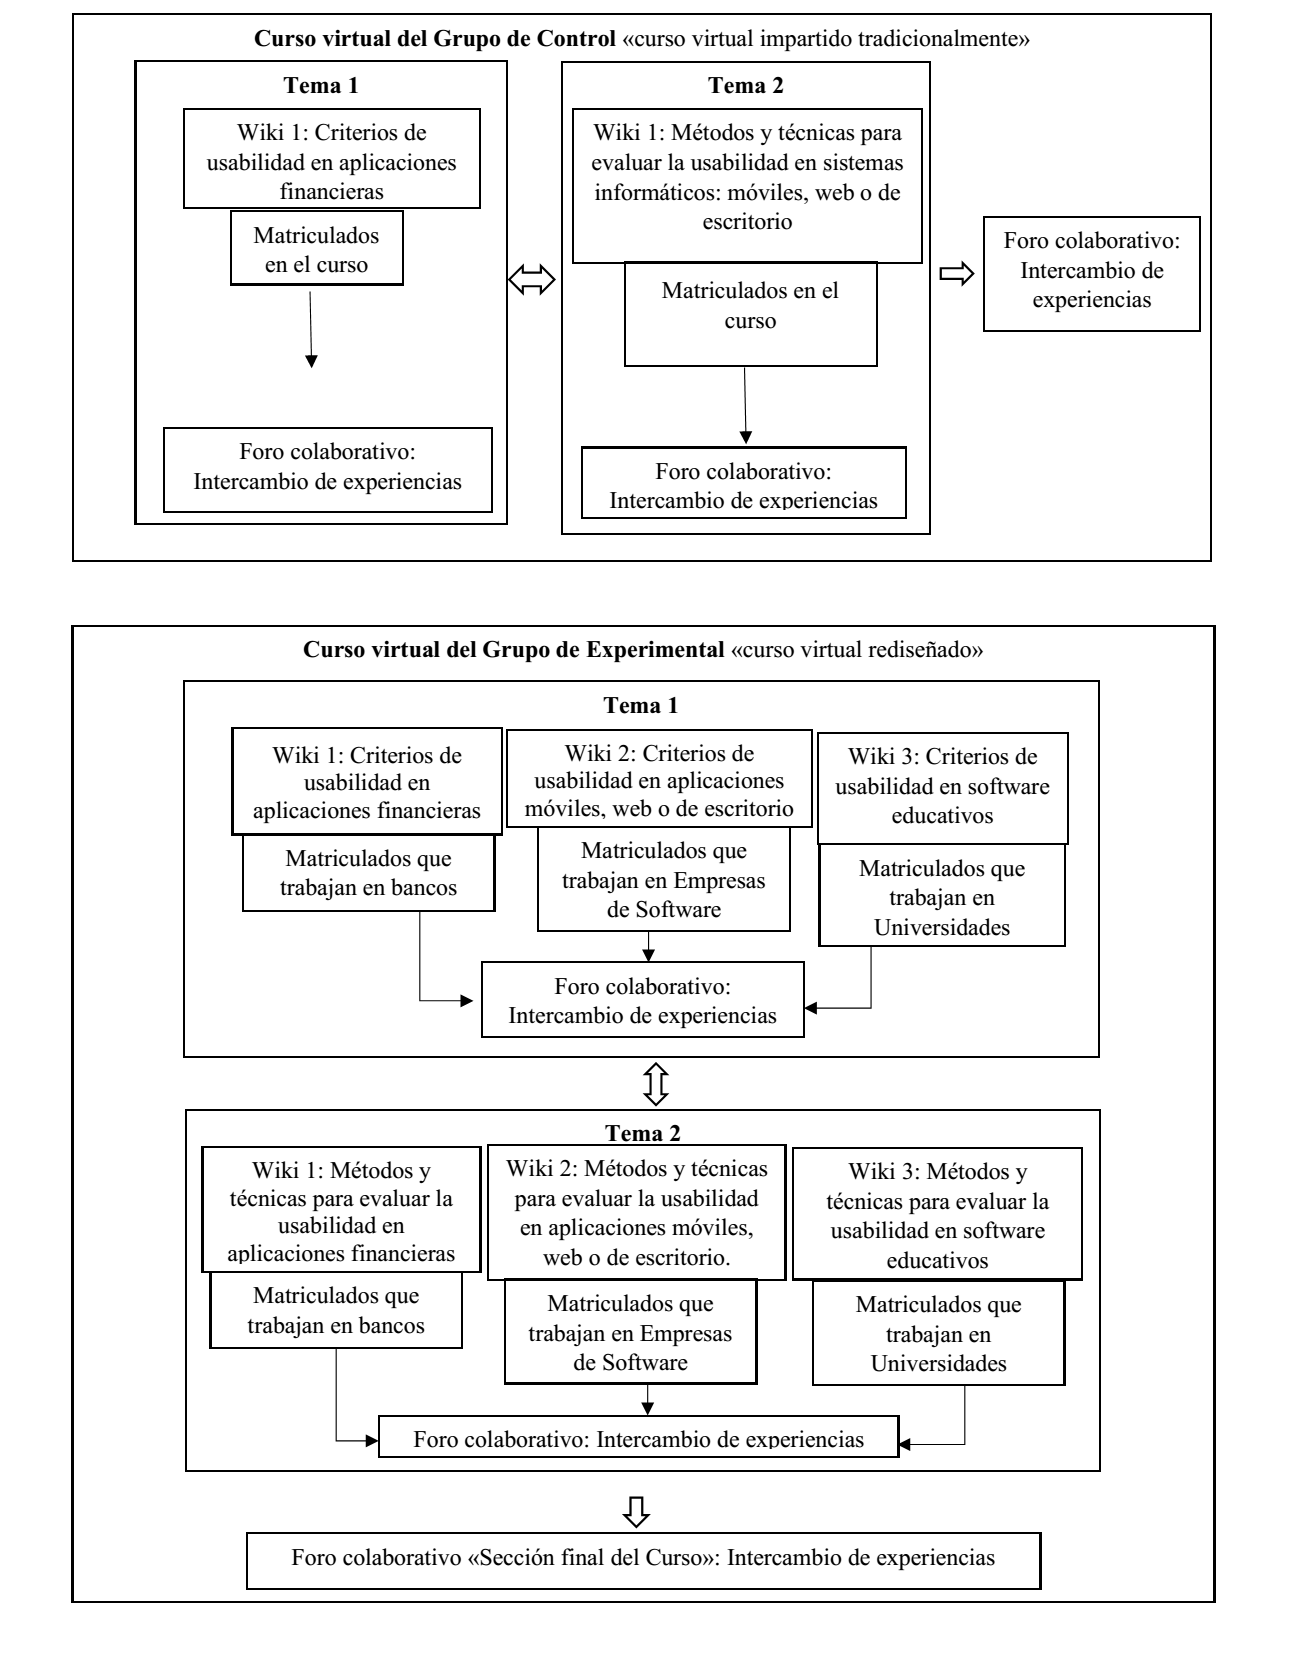
\includegraphics[width=1\textwidth]{fig1.png}
 \caption{Procedimiento general de la investigación y características de la muestra.}
 \label{fig1}
 \source{Elaboración propia.}
\end{figure}

\begin{figure}[htbp]
 \centering
 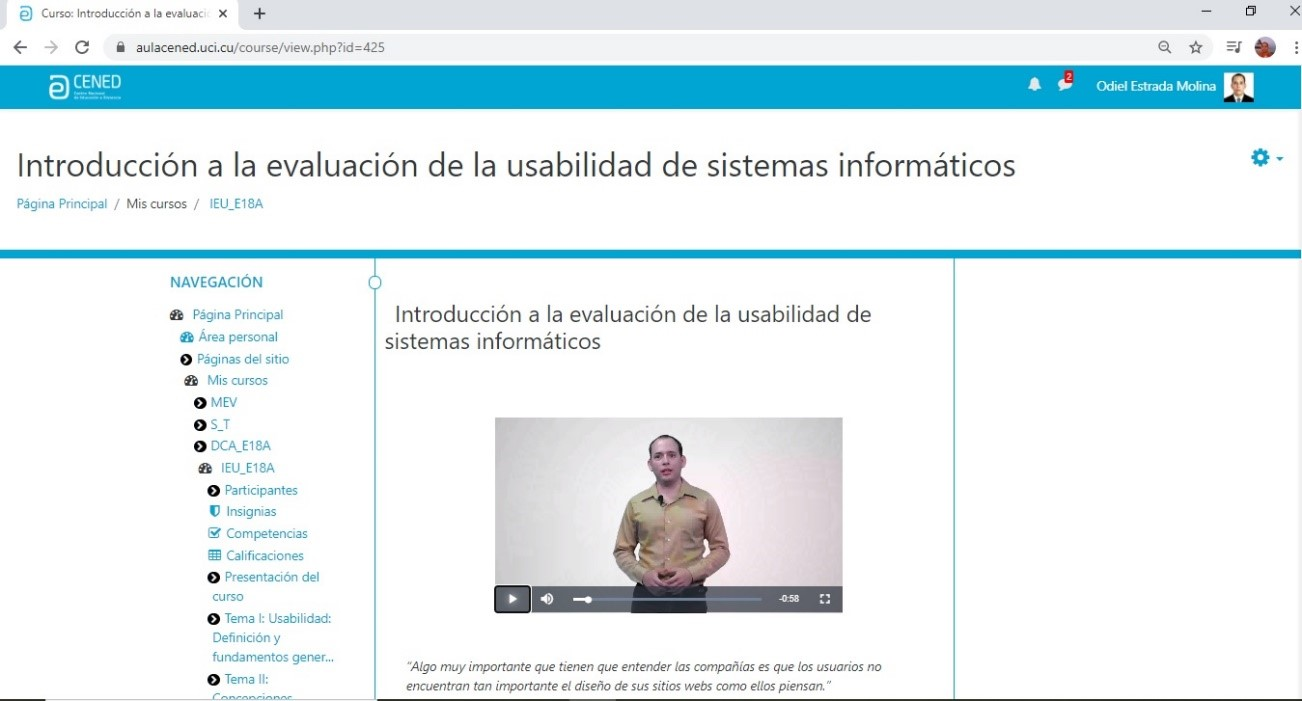
\includegraphics[width=0.7\textwidth]{fig2.png}
 \caption{Imagen del curso.}
 \label{fig2}
 \source{Elaboración propia.}
\end{figure}

\begin{table}[htbp]
\caption{Introducción a la evaluación de la usabilidad: Programación semanal.}
\label{tab1}
\centering
\begin{tabular}{p{0.15\textwidth}p{0.15\textwidth}p{0.60\textwidth}}
\toprule
Periodo  & Unidad  & Contenido de aprendizaje
\\
\midrule
\arrayrulecolor[gray]{.7}
Semana 1 & Unidad 1. & 
Fundamentos teóricos:
\begin{itemize}
    \item Definiciones de usabilidad; estándares ISO; Ingeniería de la usabilidad. Interacción Humano-Computador, Experiencia de Usuario y Usabilidad.
    \item Características, atributos y sub características genéricas de la usabilidad en productos informáticos.
    \item Características, atributos y subcaracterísticas específicas de la usabilidad en productos informáticos (comercio electrónico, tecnología educativa y sistemas de gestión de información, entre otros).
\end{itemize} \\
\midrule
%\multirow{4}{*}{Semana 1} & \multirow{4}{*}{Unidad 1.} & Fundamentos teóricos:\\
% & & Definiciones de usabilidad; estándares ISO; Ingeniería de la usabilidad. Interacción Humano-Computador, Experiencia de Usuario y Usabilidad. \\
% & & Características, atributos y sub características genéricas de la usabilidad en productos informáticos. \\
% & & Características, atributos y subcaracterísticas específicas de la usabilidad en productos informáticos (comercio electrónico, tecnología educativa y sistemas de gestión de información, entre otros). \\
Semana 2 & \multirow{3}{*}{Unidad 2.} & Métodos, técnicas e instrumentos para evaluar la usabilidad \\
Semana 3 & & Laboratorios especializados e intercambios con especialistas: aplicación de métodos, técnicas e instrumentos para evaluar la usabilidad. \\
Semana 4 & & Transformación laboral (escenario laboral de cada estudiante de posgrado): Aplicación de métodos, técnicas e instrumentos para evaluar la usabilidad. Elaboración de propuestas de mejoras (informe técnico) para mejorar la usabilidad en un producto informático. \\
\arrayrulecolor{black}
\bottomrule
\end{tabular}
\source{Elaboración propia.}
\end{table}

\begin{figure}[htbp]
 \centering
 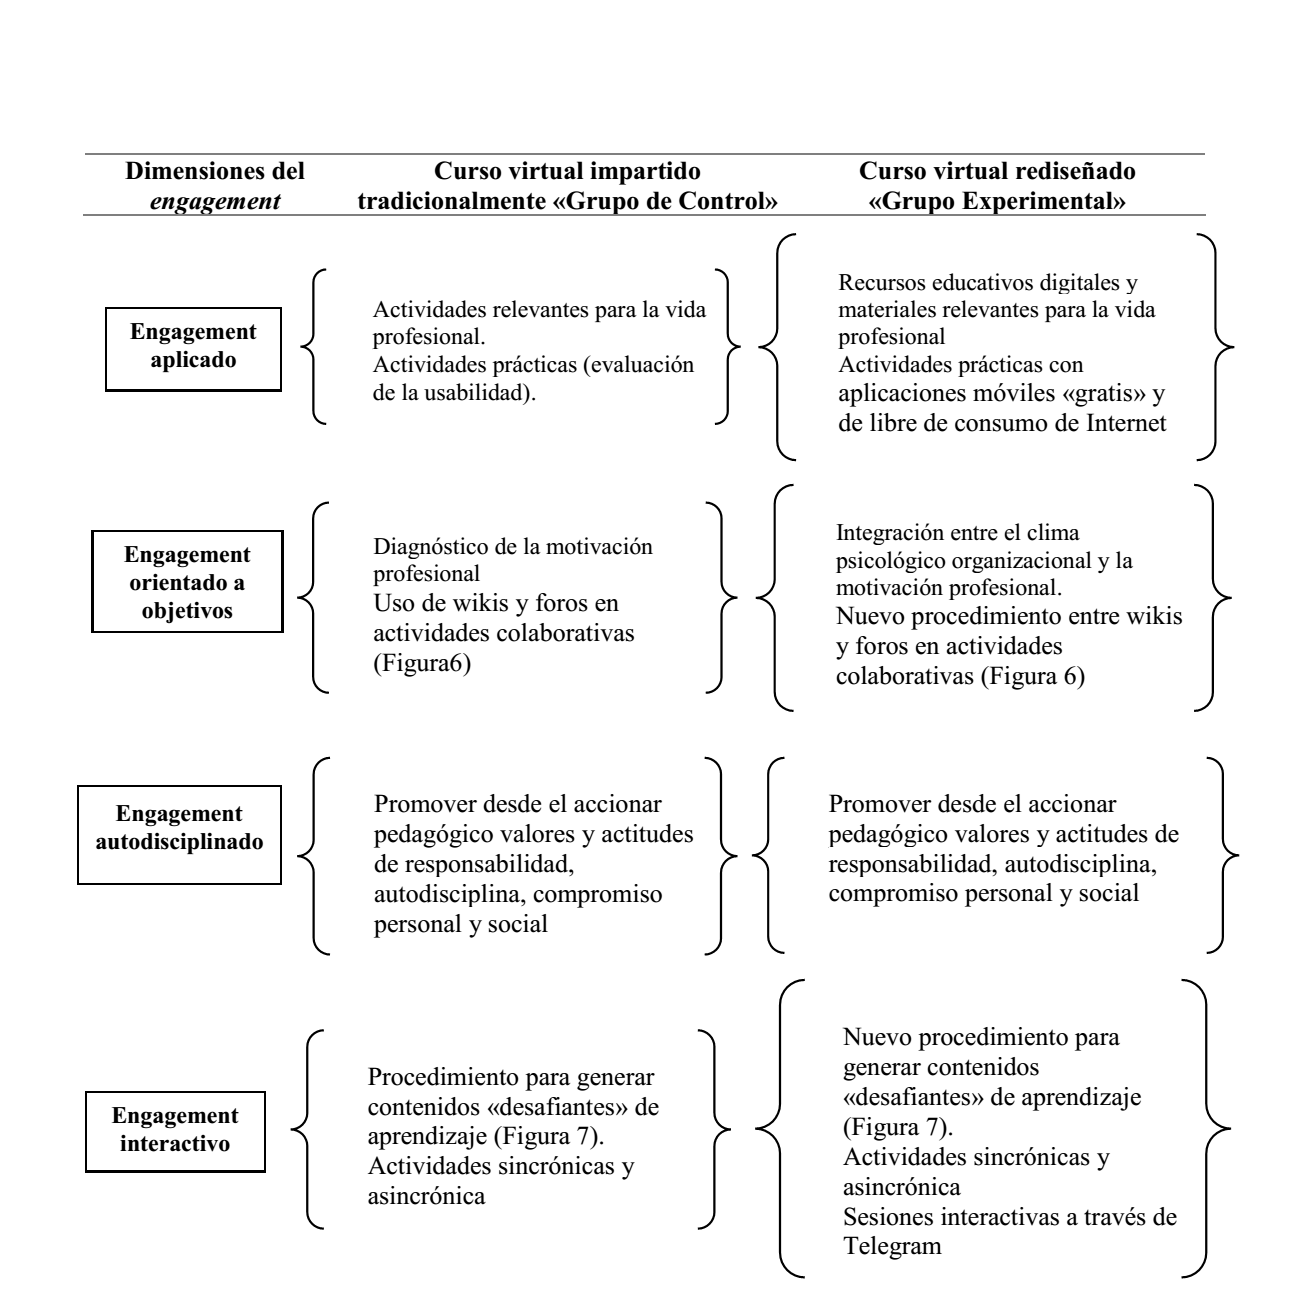
\includegraphics[width=1\textwidth]{fig3.png}
 \caption{Diseño general para promover el \emph{engagement} en el curso virtual.}
 \label{fig3}
 \source{Elaboración propia.}
\end{figure}

En el cuasi-experimento participaron 93 estudiantes (47 en el grupo experimental y 46 en el grupo de control). Esta cantidad representa el 100\% de los matriculados en el curso Introducción a la Evaluación de la Usabilidad de Sistemas Informáticos en su edición de diciembre de 2020. Se dividen en 40 mujeres (43.01\%) y 53 hombres (56.99\%). La media de edad de los alumnos es de 27 años con una desviación estándar de 3.78. Los grupos (experimental y control) son equivalentes, debido a que se seleccionaron sus miembros bajo los supuestos de la \emph{aleatoriedad}, la primera mitad para el grupo experimental y los restantes para el de control. Para esta división se tuvo en cuenta el listado ordenado por orden alfabético del primer apellido. La diferencia entre ambos grupos radica en que el de control recibió el curso tal y como ha estado diseñado en ediciones anteriores (manera tradicional) y el grupo experimental recibió el curso según el rediseño realizado.

\section{Resultados}
\subsection{Rediseño del curso virtual}
En el rediseño del curso virtual (\Cref{tab2}) se elaboraron nuevos procedimientos colaborativos \Cref{fig4} e \Cref{fig5} los cuales son explicados en la sección de discusión a partir de los factores que determinan el \emph{engagement}.

\begin{table}[htbp]
\caption{Comparaciones entre el diseño del curso del grupo de control y del experimental.}
\label{tab2}
\centering
\begin{tabular}{p{0.08\textwidth}p{0.25\textwidth}p{0.25\textwidth}p{0.25\textwidth}}
\toprule
Temas 
& Recursos educativos digitales y tipo de actividades 
& Curso virtual impartido tradicionalmente «Grupo de Control» 
& Curso virtual rediseñado «Grupo Experimental» 
\\ 
\midrule
Tema I 
& \multirow{2}{=}{Foros, Chat, Wiki, recursos multimedia, objetos de aprendizaje, mapas conceptuales y tareas} 
& \multirow{2}{=}{Procedimiento colaborativo tradicional \cite{bakker2018, mohd2020, eltahir2021, sim2021, walker2021, smith2021}} %(BAKKER; PETROU; OP DEN KAMP; TIMS, 2018; MOHD; JANIKOWSKI; GUYKER; WANG, 2020; ELTAHIR; ALSALHI; AL-QATAWNEH; JARADAT, 2021; SIM; PHEK-LIN; HANNAH; CHENG-SIM, 2021; WALKER; KORALESKY, 2021; SMITH; BOSCAK, 2021)
& \multirow{2}{=}{
-- Nuevo procedimiento colaborativo (\Cref{fig3,fig4}) \newline
-- Empleo del Telegram
} \\
Tema II & & & \\[22ex]
\toprule
\multicolumn{4}{c}{Procedimiento didáctico-metodológico}
\\
\midrule
\arrayrulecolor[gray]{.7}
\multicolumn{2}{p{0.33\textwidth}}{
Curso virtual impartido tradicionalmente «Grupo de Control» } &
\multicolumn{2}{p{0.5\textwidth}}{Curso virtual rediseñado «Grupo Experimental» }\\
\midrule
\multicolumn{2}{p{0.33\textwidth}}{
Guías didácticas, metodologías, tutorías, asesoría, contenido didáctico y formas de evaluación en función a las tendencias actuales de la industria del software. } & 
\multicolumn{2}{p{0.5\textwidth}}{
-- Se incluye un nuevo procedimiento basado en la interacción con los directivos y jefes de los profesionales matriculados en el curso y que se encuentran en confinamiento en sus casas. \newline
-- Guías didácticas, guías metodologías, tutorías, asesoría, contenido didáctico y formas de evaluación en función a las tendencias actuales de la industria del software.
} \\
\arrayrulecolor{black}
\bottomrule
\end{tabular}
\source{Elaboración propia.}
\end{table}

\begin{figure}[htbp]
 \centering
 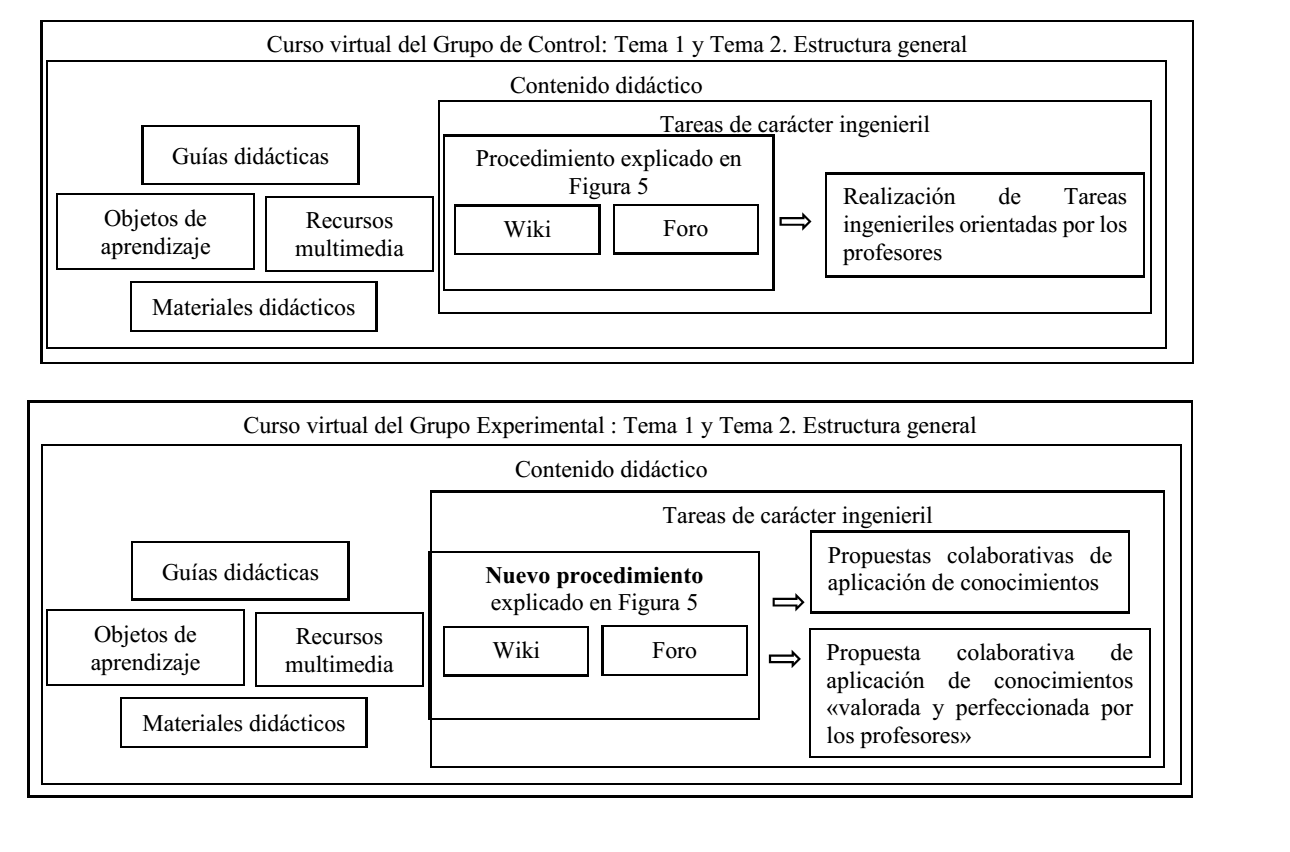
\includegraphics[width=1\textwidth]{fig4.png}
 \caption{Estructura general del contenido didáctico en los dos cursos virtuales.}
 \label{fig4}
 \source{Elaboración propia.}
\end{figure}

\begin{figure}[htbp]
 \centering
 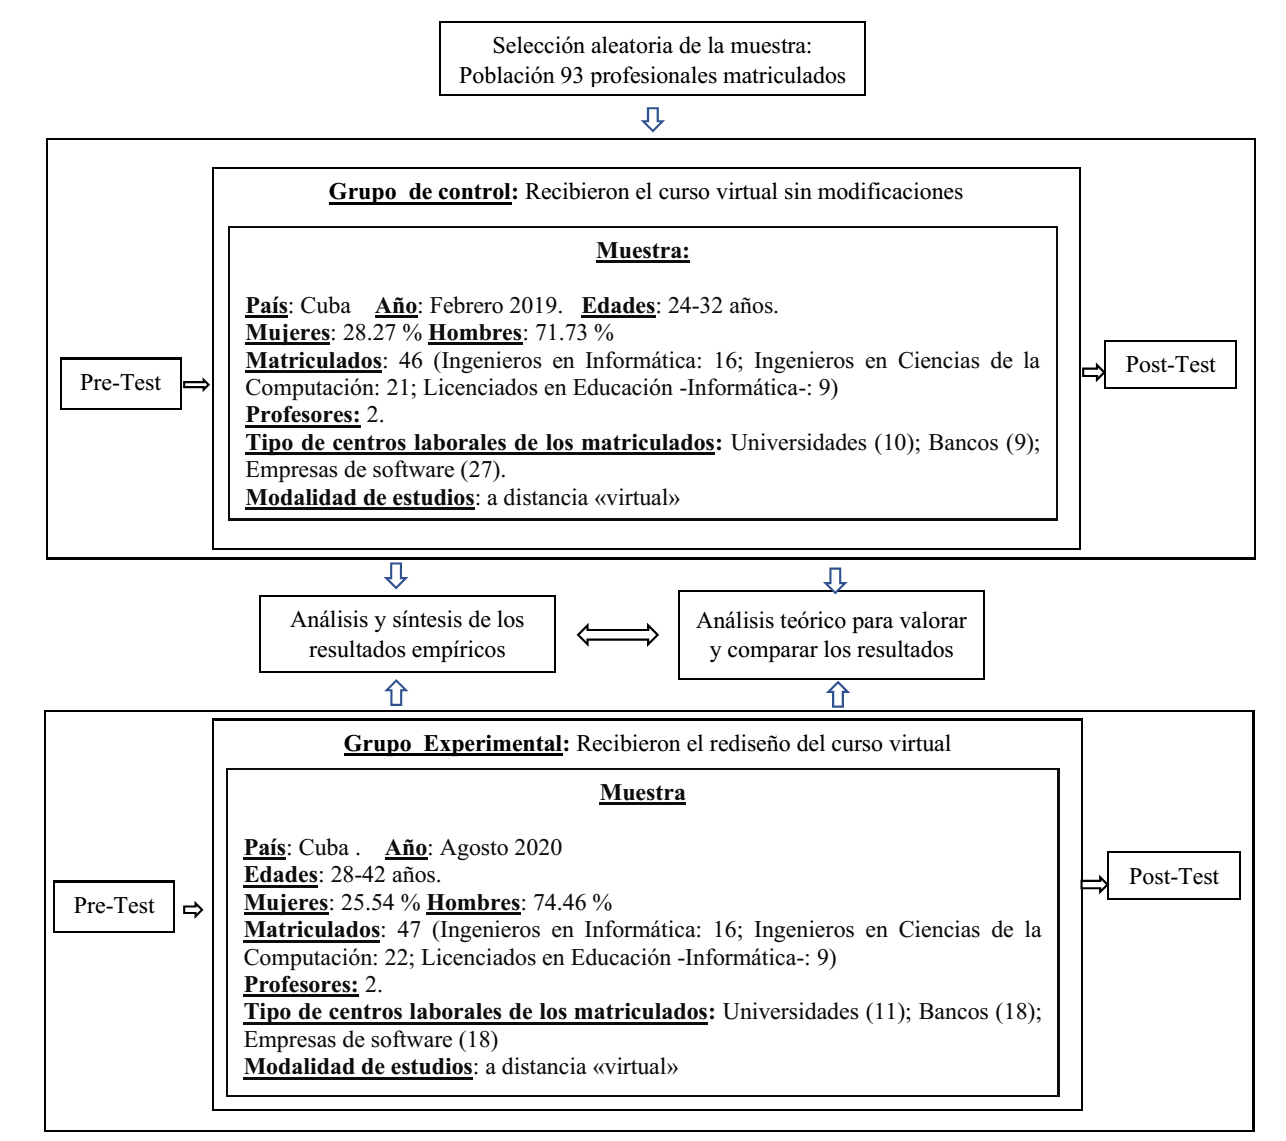
\includegraphics[width=1\textwidth]{fig5.png}
 \caption{Relación entre los wikis y foros en actividades colaborativas.}
 \label{fig5}
 \source{Elaboración propia.}
\end{figure}

\subsection{Resultados del cuasi-experimento}
Estos resultados están asociados a la pregunta de investigación. ¿El rediseño del curso virtual Introducción a la Evaluación de la Usabilidad de Sistemas Informáticos propicia mayores niveles de \emph{engagement} en las actuales condiciones de confinamiento provocado por la pandemia Covid-19 en Cuba?

Para ello se planteó la siguiente hipótesis:
\begin{itemize}
    \item H0: No se observan cambios entre la puntuación media obtenida en la evaluación pre y post-test con el cuestionario para medir \emph{engagement} en los cursos virtuales en el grupo que realiza el experimento, a un nivel de significación del 0,05.
\end{itemize}

A continuación, se muestran en la \Cref{tab3} los resultados obtenidos al analizar la puntuación media de los factores del cuestionario. Se observa en los cuatro factores la puntuación inicial y final de los dos grupos. Cada puntuación de los factores sigue una distribución normal. Esto se debe a que los valores de significatividad de la prueba de normalidad Kolmogorov-Smirnov son todos mayores a 0.05 (en este caso .142 < p > .264). En todos los casos el grupo experimental aumenta en al menos un punto la media de cada factor, sin embargo no sucede así en el grupo de control. Se realizaron las pruebas correspondientes para estudiar si la diferencia que presenta el grupo experimental se puede considerar estadísticamente significativa. Se ha aplicado la prueba de comparación de medias para muestras relacionadas.

\begin{table}[htbp]
\caption{Media de los factores del Cuestionario en el cuasi-experimento.}
\label{tab3}
\centering
\begin{tabular}{lllll}
\toprule
Factor &  & Media & N & DE \\ 
\midrule
\arrayrulecolor[gray]{.7}
\multirow{4}{*}{\emph{Engagement} aplicado} & GC\_Pre & 3.12 & 46 & 0.78 \\
 & GC\_Post & 3.37 & 46 & 0.83 \\
 \cmidrule{2-5}
 & GE\_Pre & 3.09 & 47 & 0.97 \\
 & GE\_Post & 4.12 & 47 & 0.23 \\
\midrule
\multirow{4}{*}{\emph{Engagement} orientado a objetivos} & GC\_Pre & 3.28 & 46 & 0.89 \\
 & GC\_Post & 3.24 & 46 & 0.91 \\
 \cmidrule{2-5}
 & GE\_Pre & 3.37 & 47 & 0.78 \\
 & GE\_Post & 4.52 & 47 & 0.24 \\
\midrule
\multirow{4}{*}{\emph{Engagement} autodisciplinado} & GC\_Pre & 2.98 & 46 & 1.12 \\
 & GC\_Post & 3.12 & 46 & 0.84 \\
 \cmidrule{2-5}
 & GE\_Pre & 3.03 & 47 & 0.93 \\
 & GE\_Post & 4.15 & 47 & 0.31 \\
\midrule
\multirow{4}{*}{\emph{Engagement} interactivo} & GC\_Pre & 3.49 & 46 & 0.69 \\
 & GC\_Post & 3.38 & 46 & 0.89 \\
 \cmidrule{2-5}
 & GE\_Pre & 3.37 & 47 & 0.95 \\
 & GE\_Post & 4.59 & 47 & 0.31 \\
\arrayrulecolor{black}
\bottomrule
\end{tabular}
\source{Elaboración propia.}
\end{table}

La \Cref{tab4} indica el resultado del análisis de comparación entre medias, donde se muestran la diferencia de medias y los resultados obtenidos de la aplicación de la prueba t de Student y la probabilidad asociada al valor t. Se utiliza esta prueba debido a la normalidad de los datos, previamente demostrada. Se muestra el tamaño del efecto y su estimación mediante r.

\begin{table}[htbp]
\caption{Resultado del análisis de comparación entre medias.}
\label{tab4}
\centering
\begin{tabular}{p{0.2\textwidth}llllll}
\toprule
Factor &   & Media & t & Sig & \multicolumn{1}{>{\raggedright}p{0.15\textwidth}}{Tamaño del efecto (d de Cohen)} & \multicolumn{1}{>{\raggedright}p{0.15\textwidth}}{Estimación del tamaño del efecto mediante r} \\
\midrule
\arrayrulecolor[gray]{.7}
\multirow{4}{=}{\emph{Engagement} aplicado} & 
GC\_Pre & \multirow{2}{*}{0.25} & \multirow{2}{*}{-0.234} & \multirow{2}{*}{.298} & \multirow{2}{*}{-0.031} & \multirow{2}{*}{-0.15} \\ & GC\_Post \\
\cmidrule{2-7} &
GC\_Pre & \multirow{2}{*}{1.03} & \multirow{2}{*}{-2.987} & \multirow{2}{*}{.000} & \multirow{2}{*}{-1.461} & \multirow{2}{*}{-0.58} \\ & GC\_Post \\
\midrule
\multirow{4}{=}{\emph{Engagement} orientado a objetivos} & 
GC\_Pre & \multirow{2}{*}{-0.04} & \multirow{2}{*}{-0.397} & \multirow{2}{*}{.131} & \multirow{2}{*}{0,044} & \multirow{2}{*}{0.02} \\ & GC\_Post \\ 
\cmidrule{2-7} &
GC\_Pre & \multirow{2}{*}{1.15} & \multirow{2}{*}{-3.049} & \multirow{2}{*}{.000} & \multirow{2}{*}{-1.992} & \multirow{2}{*}{-0.70} \\ & GC\_Post \\
\midrule
\multirow{4}{=}{\emph{Engagement} autodisciplinado} & 
GC\_Pre & \multirow{2}{*}{0.14} &\multirow{2}{*}{-0.431} &\multirow{2}{*}{.241} &\multirow{2}{*}{-0.141} &\multirow{2}{*}{-0.07}\\ & GC\_Post \\ 
\cmidrule{2-7} &
GC\_Pre & \multirow{2}{*}{1.12} &\multirow{2}{*}{-2.661} &\multirow{2}{*}{.000} &\multirow{2}{*}{3.069} &\multirow{2}{*}{0.83}\\ & GC\_Post \\
\midrule
\multirow{4}{=}{\emph{Engagement} interactivo} & 
GC\_Pre & \multirow{2}{*}{-0.11} &\multirow{2}{*}{-0.129} &\multirow{2}{*}{.198} &\multirow{2}{*}{0,138} &\multirow{2}{*}{0.06}\\ & GC\_Post \\ 
\cmidrule{2-7} &
GC\_Pre & \multirow{2}{*}{1.12} &\multirow{2}{*}{-3.792} &\multirow{2}{*}{.000} &\multirow{2}{*}{-1.726} &\multirow{2}{*}{0.65}\\ & GC\_Post \\
\arrayrulecolor{black}
\bottomrule
\end{tabular}
\source{Elaboración propia.}
\centering
\end{table}

Se observa que el grupo experimental aumentó sus niveles de \emph{engagement} en el curso virtual después de su rediseño, siendo en cada caso su diferencia significativa a un nivel de confianza de 95\% ($\alpha = .05$). En el grupo de control ningún valor fue significativo. Por tal motivo se rechaza la hipótesis H0 y se acepta el hecho de que sí existen diferencias significativas entre la puntuación media obtenida en la evaluación pre y post-test con el Cuestionario para medir \emph{engagement} en los cursos virtuales según sus cuatro factores \cite{mohd2020}. %(MOHD; JANIKOWSKI; GUYKER; WANG, 2020).
En cuanto al tamaño del efecto y su estimación mediante r, se refleja una diferencia grande en el grupo experimental y no así en el grupo de control \cite{cohen1988}. %(COHEN, 1988).

\section{Discusión}
Varias investigaciones \cite{bakker2018, mohd2020, sim2021} % (BAKKER; PETROU; OP DEN KAMP; TIMS, 2018; MOHD; JANIKOWSKI; GUYKER; WANG, 2020; SIM; PHEK-LIN; HANNAH; CHENG-SIM, 2021)
abordan que, para lograr el \emph{engagement} es imprescindible la motivación profesional, el aprendizaje significativo, la interactividad, orientación por objetivos y la autodisciplina. Sin embargo, aun cuando se enuncian con términos diferentes, en su esencia se coincide en los factores: \emph{engagement} aplicado, \emph{engagement} orientado a objetivos, engagement autodisciplinado y el \emph{engagement} interactivo \cite{handelsman2005, mohd2020}. %(HANDELSMAN; BRIGGS; SULLIVAN; TOWLER, 2005; MOHD; JANIKOWSKI; GUYKER; WANG, 2020).

Ahora bien, ¿qué características debe tener un curso virtual para lograr el \emph{engagement} en las actuales condiciones de confinamiento provocado por la pandemia Covid-19?

Entorno a la pregunta 1 desde la teoría \cite{mohd2020} %(MOHD; JANIKOWSKI; GUYKER; WANG, 2020) 
son varias las características del \emph{engagement} en los cursos virtuales, por lo cual, solo se expondrán en función del rediseño elaborado. Se defienden los resultados estadísticos según los cuatros factores establecidos en la literatura científica y teniendo en cuenta los recursos tecnológicos y económicos de los países subdesarrollado como Cuba y demás países latinoamericanos \cite{murillo2020}. %(MURILLO; DUK, 2020).

\subsection{\emph{Engagement} aplicado}
Este factor expresa la relación entre los conceptos, definición y fundamentos teóricos del curso virtual y la vida profesional del estudiante generando para ello, niveles de compromiso y emoción \cite{handelsman2005, shumow2013}. % (HANDELSMAN; BRIGGS; SULLIVAN; TOWLER, 2005; SHUMOW; SCHMIDT; ZALESKI, 2013).

Las características esenciales de este factor para lograr el \emph{engagement} en el rediseño elaborado, son:

\begin{itemize}
    \item \emph{Diseño de recursos educativos digitales y materiales relevantes para la vida profesional}. Es conocida la importancia del aprendizaje significativo en la motivación profesional \cite{brown2017} %(BROWN; WHITE; BOWMAR; POWER, 2017) 
    y que a su vez, el desarrollo de materiales didácticos variados y contextualizados a diferentes escenarios laborales permite en cierto sentido, atraer y mantener la motivación \cite{elmaadaway2017}.% (ELMAADAWAY, 2017).
    
    Los resultados obtenidos en el curso virtual permiten observar la importancia de generar en el propio diseño de los recursos educativos digitales con énfasis en los audiovisuales, justificantes de la importancia que tienen las diversas aplicaciones y soluciones informáticas en los escenarios laborales en que trabajan los matriculados. A su vez la necesidad de garantizar su usabilidad desde el accionar profesional del matriculado, contribuyendo a disminuir la preocupación laboral que tienen las personas durante el confinamiento \cite{amaya2021, hernandezramos2021}. % (AMAYA; CANTÚ; MARREROS, 2021; HERNÁNDEZ-RAMOS; MARTÍNEZ-ABAD; SÁNCHEZ-PRIETO, 2021).
    
    \item \emph{Aplicación de lo aprendido}. El conocer los conceptos, la definición y los fundamentos teóricos del curso y su relación con la vida profesional del estudiante, no es suficiente para generar el \emph{engagement} aplicado, siendo necesario aplicar dichos conocimientos \cite{mohd2020}. %(MOHD; JANIKOWSKI; GUYKER; WANG, 2020). 
    Por tal motivo, la realización de actividades prácticas (evaluación de la usabilidad) en aplicaciones móviles gratis y de libre de consumo de Internet a través de una plataforma libre de distribución y actualización de aplicaciones móviles (\url{https://www.apklis.cu/}), propició que los matriculados pudieran acceder desde sus hogares mediante la Intranet Nacional. En este sentido, se elaboraron materiales didácticos que orientaban a los estudiantes que aplicaciones móviles «descargar, instalar y evaluar» en correspondencia a su escenario laboral \cite{brown2017, elmaadaway2017, davis2018, buchele2020}. %(BROWN; WHITE; BOWMAR; POWER, 2017; ELMAADAWAY, 2017; DAVIS; SRIDHARAN; KOEPKE; SINGH; BOIKO, 2018;  BÜCHELE, 2020).

\end{itemize}

\subsection{\emph{Engagement} orientado a objetivos}
Este factor se centra en los objetivos del curso. El estudiante realiza la mayoría de las actividades de aprendizaje evidenciado responsabilidad y compromiso. El rendimiento académico se refleja en los resultados y metas del aprendizaje del estudiantado \cite{stack2015}. %(STACK, 2015). 
Sus características fundamentales son:

\begin{itemize}
    \item \emph{Integración entre el clima psicológico organizacional y la motivación profesional}. Recientes estudios \cite{li2020} %(LI, TSAI, 2020)
    comprueban hipótesis relacionando variables del clima competitivo organizacional y educación virtual permanente de sus empleados. En coherencia con ello, el rediseño del curso virtual elaborado por los autores de esta investigación, implicó el contacto con directivos o jefes directos de los matriculados para conocer, dentro de lo posible, el estado actual de la transformación digital de los diferentes escenarios laborales y, en correspondencia a ello, diseñar actividades de aprendizaje que les permitiera a los matriculados solucionarlas en coherencia con su tradicional desempeño. Esta acción es coherente con el aprendizaje significativo \cite{cardona2015} %(CARDONA, 2015) 
    que, contextualizado al actual confinamiento que tienen algunos trabajadores propiciaron alternativas de trabajo a distancia en la solución de problemas profesionales de su propio puesto de trabajo.
    
    \item \emph{Actividades colaborativas}. Las actividades colaborativas en entornos virtuales de aprendizaje son esenciales para una adecuada interactividad fundamentalmente a través de los Foros y las Wikis \cite{lin2020}. %(LIN; REIGELUTH, 2020). 
    En esta investigación el empleo de los Foros y Wikis se diseñaron y aplicaron por grupos de trabajos según los tres escenarios laborales: universidades, bancos y empresas de software \Cref{fig1}. Primeramente, se realizaba el trabajo colaborativo a través de las wikis y posteriormente se defendía y compartía a través de los foros diseñados en el curso virtual. Esta nueva forma concebida en el rediseño del curso virtual enmarca una diferencia significativa en cuanto a la colaboración y el trabajo cooperativo \Cref{fig4}. Independientemente de aplicar un nuevo proceder para el rediseño del curso, se ratifica la importancia de mantener la dinámica grupal, el trabajo colaborativo y la motivación a partir de la orientación didáctica \cite{bakker2018, mohd2020, eltahir2021}. %(BAKKER; PETROU; OP DEN KAMP; TIMS, 2018; MOHD; JANIKOWSKI; GUYKER; WANG, 2020; ELTAHIR; ALSALHI; AL-QATAWNEH; JARADAT, 2021).

\end{itemize}

\subsection{\emph{Engagement} autodisciplinado y el \emph{engagement} interactivo}
Conciben que el estudiante del curso virtual, se siente motivado y emocionado con realizar las actividades de aprendizaje a partir de tareas motivadoras que provoquen desafíos, interacción e interactividad \cite{mohd2020} %(MOHD; JANIKOWSKI; GUYKER; WANG, 2020) 
con los profesores y la comunidad virtual (matriculados con el curso). Ello exige autodisciplina y el compromiso personal y social de realizar las actividades de aprendizaje, en este sentido, el \emph{engagement} autodisciplinado se expresa en unidad con los demás factores, pero por valoraciones metodológicas y didácticas abordaremos sus características en unidad con el \emph{engagement} interactivo que se centra en el contenido didáctico y su correcta interacción estudiante-estudiante, estudiante-contenido, estudiante-profesor.

Las características fundamentales del rediseño del curso virtual fueron:

\begin{itemize}
    \item \emph{Contenidos «desafiantes» de aprendizaje}. Para potenciar el \emph{engagement} desde el compromiso y motivación profesional, se diseñó un proceder didáctico que tiene su génesis la interactividad presente en el procedimiento elaborado \Cref{fig3}. El propio grupo de profesionales proponen qué herramientas o soluciones informáticas evaluar su usabilidad \Cref{fig5} posteriormente, los profesores valoran la propuesta y diseñan la actividad de aprendizaje en función de la sugerencia realizada por los estudiantes (profesionales matriculados). Los resultados estadísticos muestran que los matriculados en el grupo experimental muestran un mayor nivel de \emph{engagement} que los del grupo de control. En este sentido, se muestra una tendencia a fortalecer el aprendizaje colaborativo \cite{cavinato2021} %(CAVINATO; HUNTER; OTT; ROBINSON, 2021)
    desde las tareas de aprendizaje con carácter ingenieril.

    \item \emph{Actividades sincrónicas y asincrónica}.  La realización de actividades de diferentes tipologías y el empleo de multimedia de 10-15min permitió concentrar la atención de los estudiantes en la esencia de los contenidos \cite{cavinato2021}. %(CAVINATO; HUNTER; OTT; ROBINSON, 2021).
    Es interesante destacar que en ambos grupos los estudiantes valoraron la posibilidad de disminuir la cantidad de recursos educativos digitales basadas en multimedia y potenciar las sesiones interactivas \cite{alexander2018, kerimbayev2020, snyder2020, sim2021, walker2021, smith2021}. %(ALEXANDER; DEAS; LYONS, 2018; KERIMBAYEV; NURYM; AKRAMOVA;ABDYKARIMOVA, 2020; SNYDER; MILBRATH; LEE; GAUL; HIJMANS; LEAHY; MATTHEW, 2020; SIM; PHEK-LIN; HANNAH; CHENG-SIM, 2021; WALKER; KORALESKY,  2021; SMITH; BOSCAK, 2021).
    
    \item \emph{Sesiones interactivas a través de Telegram}. El empleo de las redes sociales digitales y en especial Telegram permite una mayor interactividad y privacidad entre los estudiantes y profesores \cite{gazcaherrera2020, paredes2020, fuentescancell2021}. %(GAZCA, 2020; PAREDES; CHIPIA, 2020; FUENTES-CANCELL; ESTRADA-MOLINA; DELGADO-YANES, 2021). 
    En el grupo experimental se potenció el uso de esta plataforma de mensajería y VOIP (Voz sobre protocolo de internet o Voz por protocolo de internet). Las funcionalidades del canal y bots personalizados (Telegram Bot API) permitieron contextualizar las orientaciones didácticas según el escenario laboral de los matriculados además, permitió realizar «audios llamada grupales» y no «videollamadas» funcionalidad que para la actual situación tecnológica y económica de Cuba (país subdesarrollado) en el tránsito de la pandemia fue de vital importancia. La funcionalidad del Chat de Moodle no se utilizó en el grupo experimental, pues para emplearlo, los matriculados deben acceder a toda la plataforma requiriendo una red robusta y una actualización continua del ancho de banda \cite {maphosa2020}. %(MAPHOSA; JITA; DUBE, 2020). 
\end{itemize} 

\section{Limitaciones}
Esta investigación tiene como limitación fundamental la muestra escogida. Si bien se realizó un cuasi-experimento identificándose el grupo de control y el experimental, la cantidad de participantes no es suficiente para realizar generalizaciones en cuanto a las características que deben tener un curso virtual para elevar el \emph{engagement} en tiempo de confinamiento físico. Este estudio inicial ratifica la importancia de diseñar alternativas educativas desde la virtualidad para hacer frente al confinamiento actual debido a la pandemia \cite{smith2021}. %(SMITH; BOSCAK, 2021).

La otra limitación se expresa en el procedimiento empleado para el uso de wikis y foros \Cref{fig4}. Fue pertinente aplicar este proceder pues los matriculados coincidían en cuanto al tipo de escenario laboral (profesionales de la informática que trabajaban en bancos, empresas de desarrollo de \emph{software} o universidades). Es real que no siempre será posible esta característica de poder agrupar los matriculados en función de su labor profesional. Independientemente de esta concepción, la principal recomendación que se brinda es la posibilidad de agrupar a los matriculados teniendo en cuenta algún tipo de clasificación potenciando así su \emph{engagement} desde el aprendizaje cooperativo y el colaborativo \cite{cardona2015, li2020}. %(CARDONA, 2015; LI; TSAI, 2020).

\section{Conclusiones}
La experimentación realizada permitió constatar que el rediseño del curso virtual Introducción a la Evaluación de la Usabilidad de Sistemas Informáticos propicia mayores niveles de \emph{engagement} en las actuales condiciones de confinamiento provocado por la pandemia Covid-19 en Cuba. Reflejándose en las diferencias estadísticas significativas obtenidas en el grupo experimental.

Potenciar el \emph{engagement} desde los cursos virtuales bajo el prisma de las actuales condiciones de confinamiento presentes en Cuba y las experiencias obtenidas en el cuasi-experimento, permite concluir lo siguiente:

\begin{itemize}
    \item Factor \emph{engagement} aplicado. El diseño de recursos educativos digitales y materiales relevantes para la vida profesional permitió diseñar actividades de aprendizaje que potencia el aprendizaje significado y la motivación profesional \cite{amaya2021}. %(AMAYA; CANTÚ; MARREROS, 2021).
    En este sentido, la aplicación de lo aprendido \cite{brown2017} %(BROWN; WHITE; BOWMAR; POWER, 2017) 
    a través de soluciones informáticas interactivas móviles «gratis» y de libre de consumo de Internet permitió elevar la motivación de los matriculados en el grupo experimental ya que se ajustaba a sus condiciones de conectividad actual.
    
    \item Factor \emph{engagement} orientado a objetivos. La integración entre el clima psicológico organizacional y la motivación profesional es un factor fundamental para el compromiso y motivación del estudiantado. En este sentido, la realización de entrevistas con los directivos o jefes de los profesionales matriculados en el curso, permitió elaborar actividades de aprendizaje y tareas contextualizadas al escenario laboral y en coherencia con el aprendizaje colaborativo. Se reafirma que el aprendizaje colaborativo y el significativo son elementos claves para lograr los objetivos de aprendizaje \cite{cardona2015, li2020}. %(CARDONA, 2015; LI; TSAI, 2020).
    
    \item Factores \emph{engagement} autodisciplinado y el \emph{engagement} interactivo. Diseñar actividades con contenidos «desafiantes» de aprendizaje, diversificar las actividades sincrónicas y asincrónicas en el entorno virtual (funcionalidades de Moodle) y propiciar sesiones interactivas a través de Telegram permiten que el estudiante se motive en la realización de las actividades de aprendizaje.
   
    El trabajo colaborativo \cite{cavinato2021} %(CAVINATO; HUNTER; OTT; ROBINSON,2021) 
    es fundamental para enriquecer las propuestas didácticas de evaluación, a su vez, las actividades a través de Telegram permitió a los profesores del curso crear canales y bots personalizados (Telegram Bot API) en función de los diferentes escenarios laborales además propició a los matriculados (grupo experimental) una mejor conectividad.
\end{itemize} 

Elevar el \emph{engagement} en cursos virtuales es una tarea educativa de actualidad y más en los nuevos escenarios educativos provocados por la actual pandemia Covid-19. Sin embargo, en los países subdesarrollados es creciente la brecha tecnológica y sus implicaciones educativas, por lo cual, se hace necesario diseñar alternativas para, dentro de lo posible, mantener y ofertar cursos de superación a los distintos profesionales \cite{gonzalez2020, mahdy2020, ojeda2020, santiagoiglesias2021}. %(GONZÁLEZ, 2020; MAHDY, 2020; OJEDA; ORTEGA; BOOM, 2020; SANTIAGO; HERNÁNDEZ-GARCÍA; CHAPARRO-PELÁEZ; PRIETO, 2021).

Como futuras líneas de trabajo, se propone continuar esta investigación en tres direcciones: (1) diseñar nuevos procedimientos para potenciar el \emph{engagement} en cursos virtuales; y (2)  medir el \emph{engagement} en las nuevas ediciones del curso para así comparar y llegar a posibles generalizaciones.


\printbibliography\label{sec-bib}
% if the text is not in Portuguese, it might be necessary to use the code below instead to print the correct ABNT abbreviations [s.n.], [s.l.] 
%\begin{portuguese}
%\printbibliography[title={Bibliography}]
%\end{portuguese}

\end{document}
